\documentclass[12pt,a4paper]{article}
\usepackage[utf8]{inputenc}
\usepackage[english]{babel}
%\usepackage{minted}
\usepackage{listings}
\usepackage{xcolor}
\usepackage{graphicx}

%For syntax highlighting
\definecolor{codegreen}{rgb}{0,0.6,0}
\definecolor{codegray}{rgb}{0.5,0.5,0.5}
\definecolor{codepurple}{rgb}{0.58,0,0.82}
\definecolor{backcolour}{rgb}{1,1,1}

%%Sets different parameters
\lstdefinestyle{mystyle}{
	backgroundcolor=\color{backcolour},   
    commentstyle=\color{codegreen},
    keywordstyle=\color{magenta},
    numberstyle=\tiny\color{codegray},
    stringstyle=\color{codepurple},
    basicstyle=\ttfamily\footnotesize,
    breakatwhitespace=false,         
    breaklines=true,                 
    captionpos=b,                    
    keepspaces=true,                 
    numbers=left,                    
    numbersep=5pt,                  
    showspaces=false,                
    showstringspaces=false,
    showtabs=false,                  
    tabsize=4
}
\lstset{style=mystyle}

\title{\bf String Manipulations}
\author{\vspace{-10ex}}
\date{\vspace{-10ex}}
\begin{document}
\maketitle

\begin{minipage}{0.45\textwidth}
        \begin{tabular}{l l}
            \textbf{Expt No:}&3\\
            \textbf{Date :}&11/09/2020
        \end{tabular}
\end{minipage}%
\begin{minipage}{0.45\textwidth}
        \begin{tabular}{l l}
             \textbf{Name:}& Shivanirudh S G  \\
             \textbf{Reg No:} & 185001146 
        \end{tabular}
\end{minipage}
\vspace{1cm}
\hrule

\begin{flushleft}
\subsection*{\textbf{Aim:}} 
To perform string manipulation in 8086.

\vspace{1cm}
\hrule
\subsection*{\textbf{\underline{Moving a string of bytes}}}

\subsubsection*{\textbf{Algorithm:}}
\begin{itemize}
    \item Move the data segment to the AX register and then move it to the DS register.
    \item Move the extra segment to the AX register and then move it to the ES register.
    \item Move the offset of source string to SI register. 
    \item Move the offset of destination string to the DI register. 
    \item Move the length of the string to the CX register.
    \item Clear the direction flag. 
    \item Move the string from address pointed by DS and SI to address pointed by ES and DI using REP MOVSB.
\end{itemize}

\newpage
\subsubsection*{\textbf{Program:}}

\begin{table}[htb]
\centering
\resizebox{\columnwidth}{!}{
\begin{tabular}{|l|l|} 
\hline
\textbf{Program}                                                 & \textbf{Comments}                             \\ 
\hline
\hline
assume cs:code, ds:data, es:extra                                & Declare code, data and extra segments         \\
\hline
data segment                                                     & Start of data segment                         \\
\hline 
source db 98H, 76H, 54H, 32H, 10H                                & Define array of bytes source                  \\
\hline
count dw 0005H                                                   & Define word count with hex value 0005         \\
\hline     
data ends                                                        & End of data segment                           \\
\hline
extra segment                                                    & Start of extra segment                        \\
\hline
dest db ?                                                        & Define array of bytes dest with unknown values\\
\hline
extra ends                                                       & End of extra segment                          \\
\hline
code segment                                                     & Start of code segment                         \\
\hline
start:~ mov ax, data                                             & Move data segment contents to AX register     \\ 
\hline
mov ds, ax                                                       & Move data in AX register to DS register       \\ 
\hline
mov ax, extra                                                    & Move extra segment contents to AX register    \\ 
\hline
mov es, ax                                                       & Move data in AX register to ES register       \\ 
\hline
mov si, offset source                                            & Move offset of source to SI register          \\ 
\hline
mov di, offset dest                                              & Move offset of dest to DI register            \\ 
\hline
mov cx, count                                                    & Move value of count to CX register            \\ 
\hline
cld                                                              & Clear the direction flag                      \\
\hline
rep movsb                                                        & Move contents of SI to DI till CX = 0         \\
\hline
int 21h                                                          & Request interrupt routine                     \\ 
\hline
code ends                                                        & End of code segment                           \\
\hline
end start                                                        &                                               \\
\hline
\end{tabular}
}
\end{table}

\newpage
\subsection*{\textbf{Unassembled code:}}
\begin{figure}[h]
    \centering
    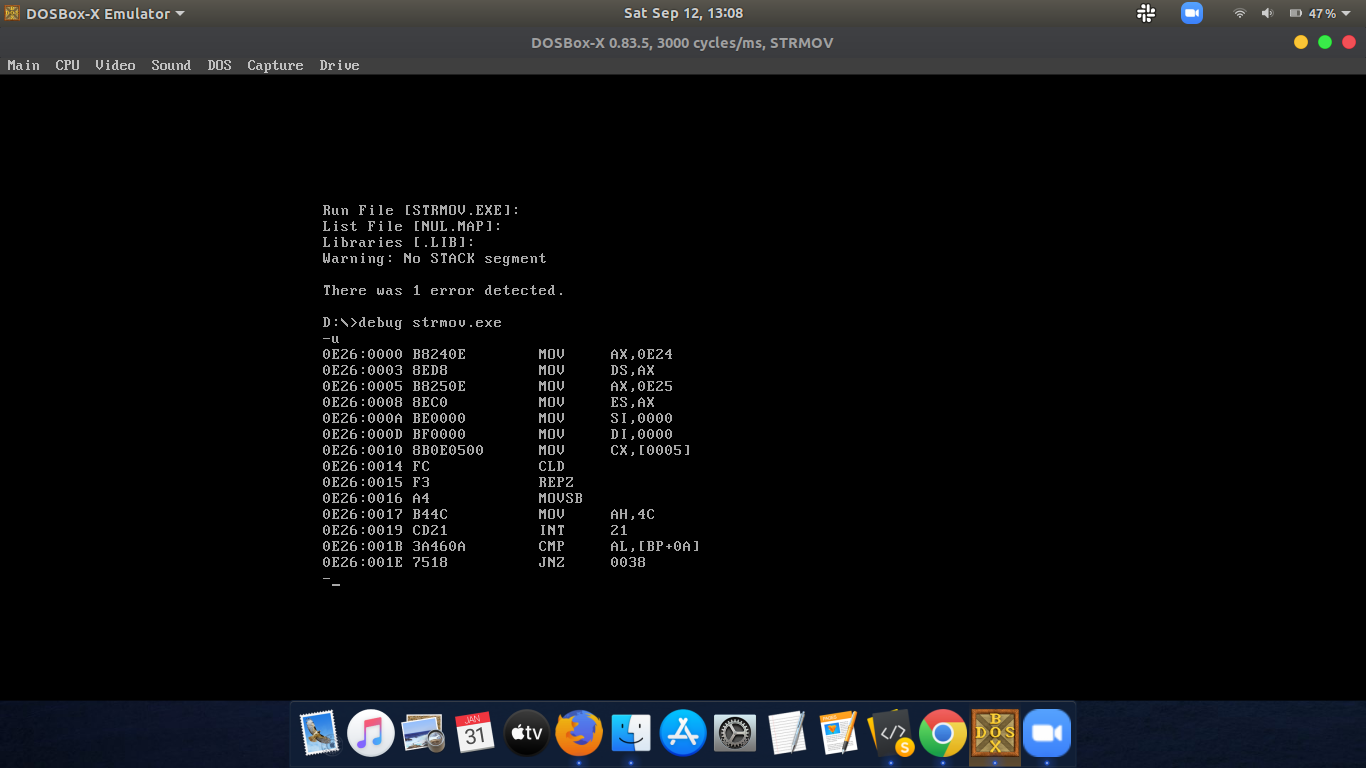
\includegraphics[trim = 100mm 60mm 200mm 120mm, clip, width = \textwidth]{Pics/StrmovUS.png}
\end{figure}
\subsubsection*{\textbf{Input and Output:}}
\begin{figure}[h]
    \centering
    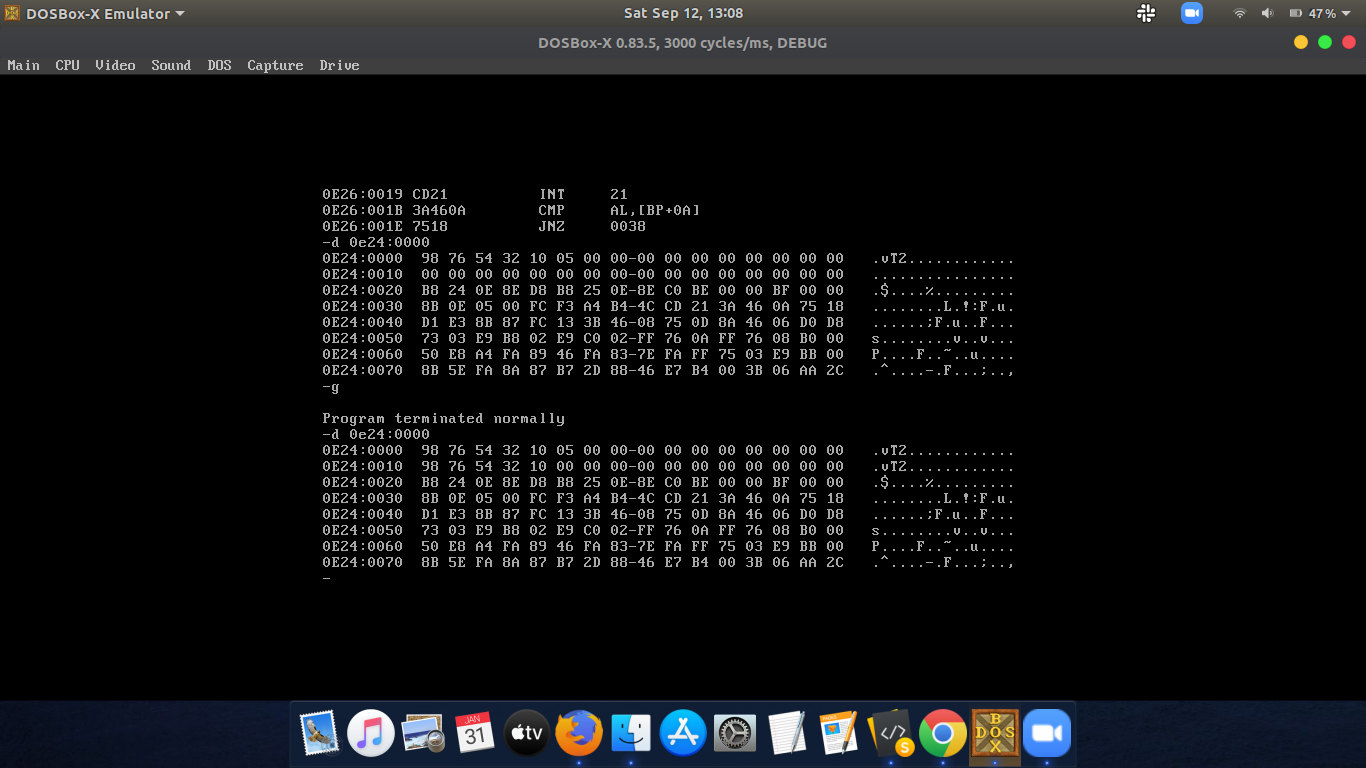
\includegraphics[trim = 100mm 60mm 100mm 80mm, clip, width = \textwidth]{Pics/StrmovIO.png}
    \caption{ \textbf{Input:} \emph{DS:} 98 76 54 32 10H, \emph{ES:} 00 00 00 00 00H; \newline \hspace{1cm}
              \textbf{Output:} \emph{DS:} 98 76 54 32 10H, \emph{ES:} 98 76 54 32 10H}
\end{figure}
%--------------------------------------------------------------------------------------------------------------------------------------------
\subsection*{\textbf{\underline{Comparing 2 strings of bytes}}}

\subsubsection*{\textbf{Algorithm:}}
\begin{itemize}
    \item Move the data segment to the AX register and then move it to the DS register.
    \item Move the extra segment to the AX register and then move it to the ES register.
    \item Move the offset of string s1 to SI register. 
    \item Move the offset of string s2 to the DI register. 
    \item Move the length of the string to the CX register. Increment value of CX.
    \item Clear the direction flag. 
    \item Compare the strings from addresses pointed by DS and SI and by ES and DI using REPE CMPSB.
    \item Move contents of cx, which now has the position in string where the difference is, to RESULT.
\end{itemize}

\newpage
\subsubsection*{\textbf{Program:}}

\begin{table}[htb]
\centering
\resizebox{\columnwidth}{!}{
\begin{tabular}{|l|l|} 
\hline
\textbf{Program}                                                 & \textbf{Comments}                             \\ 
\hline
\hline
assume cs:code, ds:data, es:extra                                & Declare code, data and extra segments         \\
\hline
data segment                                                     & Start of data segment                         \\
\hline 
s1 db 98H, 76H, 54H, 32H, 11H                                    & Define array of bytes s1                      \\
\hline
count dw 0005H                                                   & Define word count with hex value 0005         \\
\hline     
result db 00H                                                    & Define byte result with hex value 00          \\
\hline
data ends                                                        & End of data segment                           \\
\hline
extra segment                                                    & Start of extra segment                        \\
\hline
s2 db 98H, 76H, 54H, 32H, 10H                                    & Define array of bytes s2                      \\
\hline
extra ends                                                       & End of extra segment                          \\
\hline
code segment                                                     & Start of code segment                         \\
\hline
start:~ mov ax, data                                             & Move data segment contents to AX register     \\ 
\hline
mov ds, ax                                                       & Move data in AX register to DS register       \\ 
\hline
mov ax, extra                                                    & Move extra segment contents to AX register    \\ 
\hline
mov es, ax                                                       & Move data in AX register to ES register       \\ 
\hline
mov si, offset source                                            & Move offset of source to SI register          \\ 
\hline
mov di, offset dest                                              & Move offset of dest to DI register            \\ 
\hline
mov cx, count                                                    & Move value of count to CX register            \\ 
\hline
inc cx                                                           & Increment value of CX                         \\
\hline
cld                                                              & Clear the direction flag                      \\
\hline
repe cmpsb                                                       & Compare bytes of s1 and s2 till unequal       \\
\hline
mov result, cx                                                   & Move contents of CX to result                 \\
\hline
int 21h                                                          & Request interrupt routine                     \\ 
\hline
code ends                                                        & End of code segment                           \\
\hline
end start                                                        &                                               \\
\hline
\end{tabular}
}
\end{table}

\newpage
\subsection*{\textbf{Unassembled code:}}
\begin{figure}[h]
    \centering
    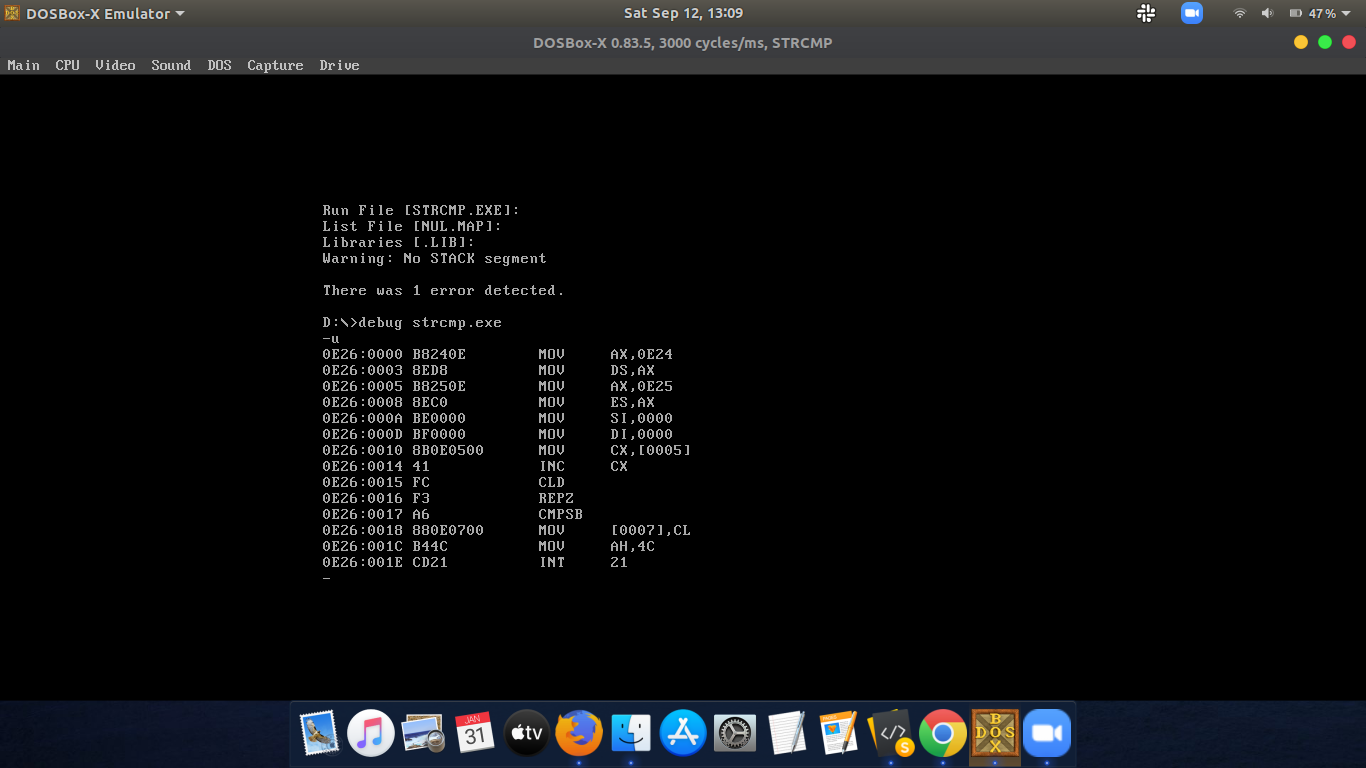
\includegraphics[trim = 100mm 60mm 200mm 120mm, clip, width = \textwidth]{Pics/StrcmpUS.png}
\end{figure}
\subsubsection*{\textbf{Input and Output:}}
\begin{figure}[h]
    \centering
    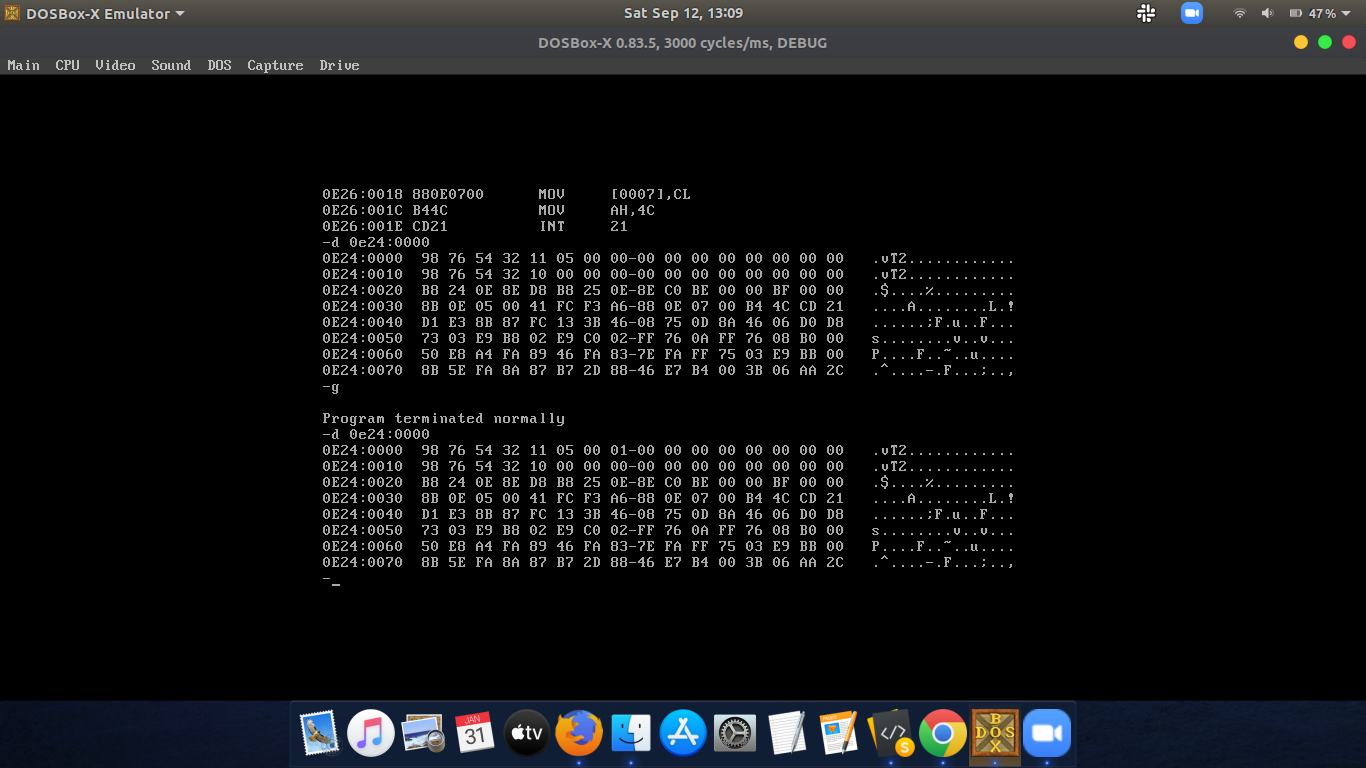
\includegraphics[trim = 100mm 60mm 100mm 80mm, clip, width = \textwidth]{Pics/StrcmpIO.png}
    \caption{ \textbf{Input:} \emph{DS:} 98 76 54 32 11H, \emph{ES:} 98 76 54 32 10H; \newline \hspace{1cm}
              \textbf{Output:} \emph{Result:} 0001 }
\end{figure}
%--------------------------------------------------------------------------------------------------------------------------------------------
\subsection*{\textbf{\underline{Searching a byte in a string}}}

\subsubsection*{\textbf{Algorithm:}}
\begin{itemize}
    \item Move the data segment to the AX register and then move it to the DS register.
    \item Move the extra segment to the AX register and then move it to the ES register.
    \item Move the offset of string to the DI register.
    \item Move the byte to be searched to the AL register. 
    \item Move the length of the string to the CX register. Increment value of CX
    \item Clear the direction flag. 
    \item Scan the string for the specified byte using REPNE SCASB.
    \item Move contents of CX register, which now has location of the specified byte in the string, to RESULT.
\end{itemize}

\newpage
\subsubsection*{\textbf{Program:}}

\begin{table}[htb]
\centering
\resizebox{\columnwidth}{!}{
\begin{tabular}{|l|l|} 
\hline
\textbf{Program}                                                 & \textbf{Comments}                             \\ 
\hline
\hline
assume cs:code, ds:data, es:extra                                & Declare code, data and extra segments         \\
\hline
data segment                                                     & Start of data segment                         \\
\hline 
val db 32H                                                       & Define byte val with hex value 32             \\
\hline
count dw 0005H                                                   & Define word count with hex value 0005         \\
\hline 
result dw 0000H                                                  & Define word result with hex value 0000        \\
\hline    
data ends                                                        & End of data segment                           \\
\hline
extra segment                                                    & Start of extra segment                        \\
\hline
str db 98H, 76H, 54H, 32H, 10H                                   & Define array of bytes dest with unknown values\\
\hline
extra ends                                                       & End of extra segment                          \\
\hline
code segment                                                     & Start of code segment                         \\
\hline
start:~ mov ax, data                                             & Move data segment contents to AX register     \\ 
\hline
mov ds, ax                                                       & Move data in AX register to DS register       \\ 
\hline
mov ax, extra                                                    & Move extra segment contents to AX register    \\ 
\hline
mov es, ax                                                       & Move data in AX register to ES register       \\ 
\hline
mov di, offset str                                               & Move offset of str to DI register             \\ 
\hline
mov al, val                                                      & Move value of val to AL register              \\
\hline
mov cx, count                                                    & Move value of count to CX register            \\ 
\hline
inc cx                                                           & Increment value of CX                         \\
\hline
cld                                                              & Clear the direction flag                      \\
\hline
repne scasb                                                      & Scan contents of DI for AL till CX = 0        \\
\hline
mov result, cx                                                   & Move contents of CX to result                 \\
\hline
int 21h                                                          & Request interrupt routine                     \\ 
\hline
code ends                                                        & End of code segment                           \\
\hline
end start                                                        &                                               \\
\hline
\end{tabular}
}
\end{table}

\newpage
\subsection*{\textbf{Unassembled code:}}
\begin{figure}[h]
    \centering
    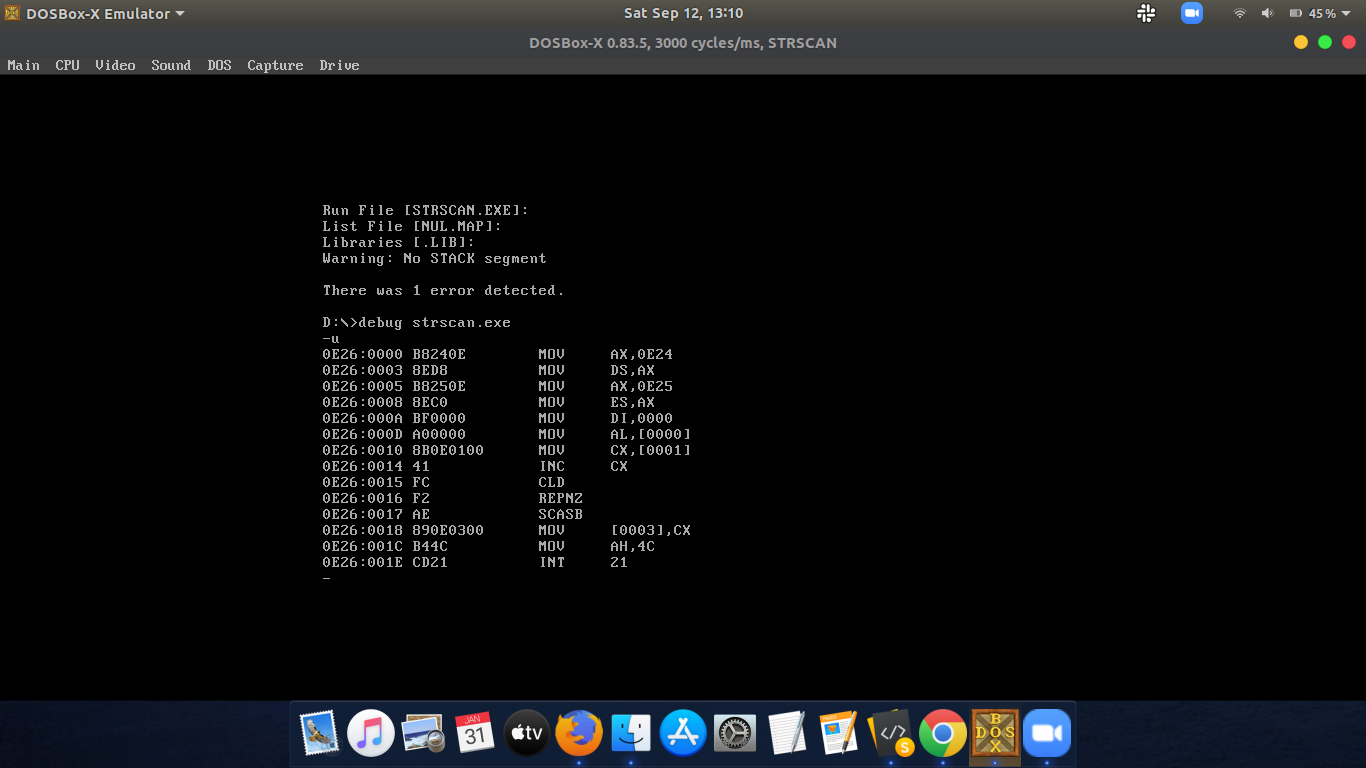
\includegraphics[trim = 100mm 60mm 200mm 120mm, clip, width = \textwidth]{Pics/StrscanUS.png}
\end{figure}
\subsubsection*{\textbf{Input and Output:}}
\begin{figure}[h]
    \centering
    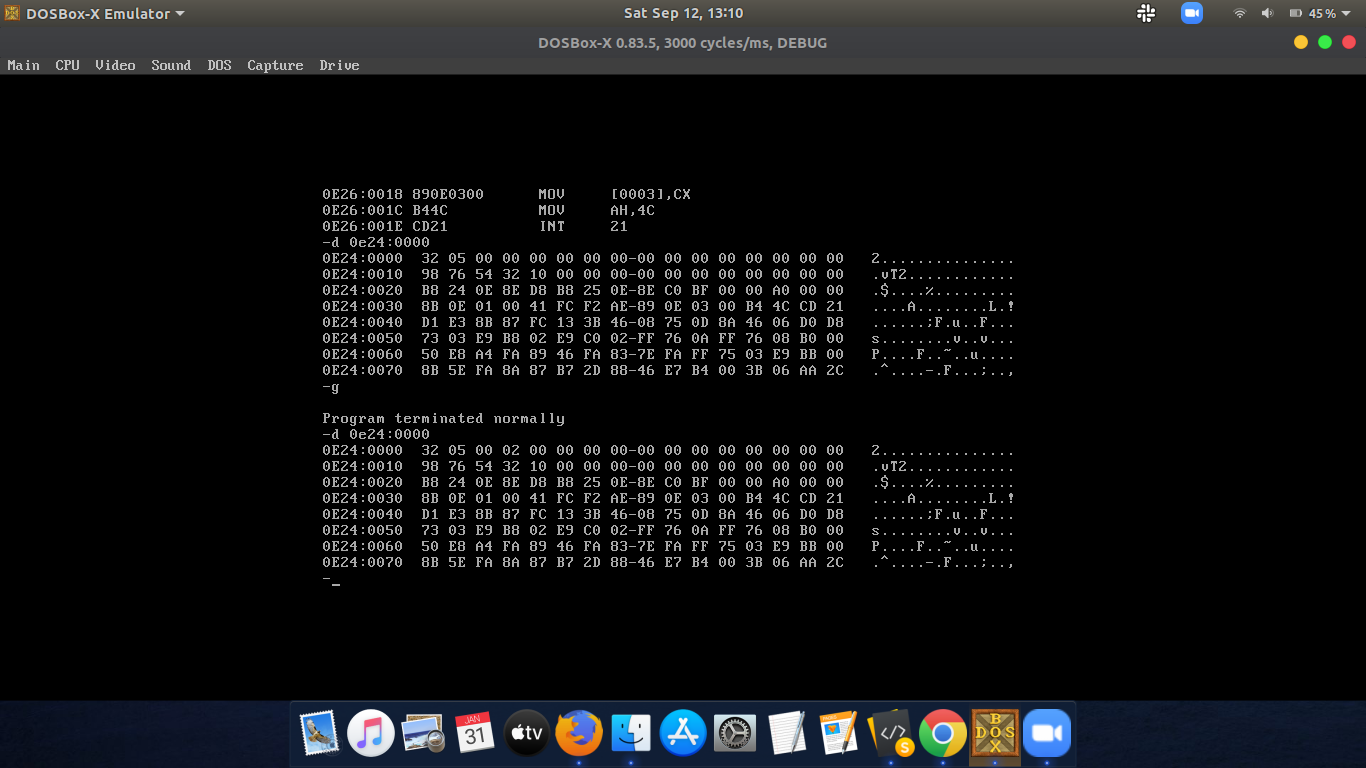
\includegraphics[trim = 100mm 60mm 100mm 80mm, clip, width = \textwidth]{Pics/StrscanIO.png}
    \caption{ \textbf{Input:} \emph{DS:} Value: 32H, \emph{ES:} 98 76 54 32 10H; \newline \hspace{1cm}
              \textbf{Output:} \emph{Result:} 0002H}
\end{figure}
%--------------------------------------------------------------------------------------------------------------------------------------------
\subsection*{\textbf{\underline{Moving a string without using string instructions}}}

\subsubsection*{\textbf{Algorithm:}}
\begin{itemize}
    \item Move the data segment to the AX register and then move it to the DS register.
    \item Move the offset of source string to the SI register.
    \item Move the offset of destination string to the DI register.
    \item Move the length of the string to the CX register. 
    \item Repeat till CX is 0:
    \begin{itemize}
        \item Move content of SI to BL, and then to DI.
        \item Increment SI, DI.
        \item Decrement CX.
    \end{itemize}
\end{itemize}

\newpage
\subsubsection*{\textbf{Program:}}

\begin{table}[htb]
\centering
\resizebox{\columnwidth}{!}{
\begin{tabular}{|l|l|} 
\hline
\textbf{Program}                                                 & \textbf{Comments}                             \\ 
\hline
\hline
assume cs:code, ds:data                                          & Declare code and data segments                \\
\hline
data segment                                                     & Start of data segment                         \\
\hline 
source db 98H, 76H, 54H, 32H, 10H                                & Define array of bytes source                  \\
\hline
count dw 0005H                                                   & Define word count with hex value 0005         \\
\hline  
dest db ?                                                        & Define array of bytes dest with unknown values\\
\hline  
data ends                                                        & End of data segment                           \\
\hline
code segment                                                     & Start of code segment                         \\
\hline
start:~ mov ax, data                                             & Move data segment contents to AX register     \\ 
\hline
mov ds, ax                                                       & Move data in AX register to DS register       \\ 
\hline
mov si, offset source                                            & Move offset of source to SI register          \\ 
\hline
mov di, offset dest                                              & Move offset of dest to DI register            \\ 
\hline
mov cx, count                                                    & Move value of count to CX register            \\ 
\hline
here:~ mov bl, [si]                                              & Move contents of SI to BL register            \\
\hline
mov [di], bl                                                     & Move contents of BL register to DI            \\
\hline
inc si                                                           & Increment value of SI                         \\
\hline
inc di                                                           & Increment value of DI                         \\
\hline
dec cx                                                           & Decrement value of CX                         \\
\hline
int 21h                                                          & Request interrupt routine                     \\ 
\hline
code ends                                                        & End of code segment                           \\
\hline
end start                                                        &                                               \\
\hline
\end{tabular}
}
\end{table}

\newpage
\subsection*{\textbf{Unassembled code:}}
\begin{figure}[h]
    \centering
    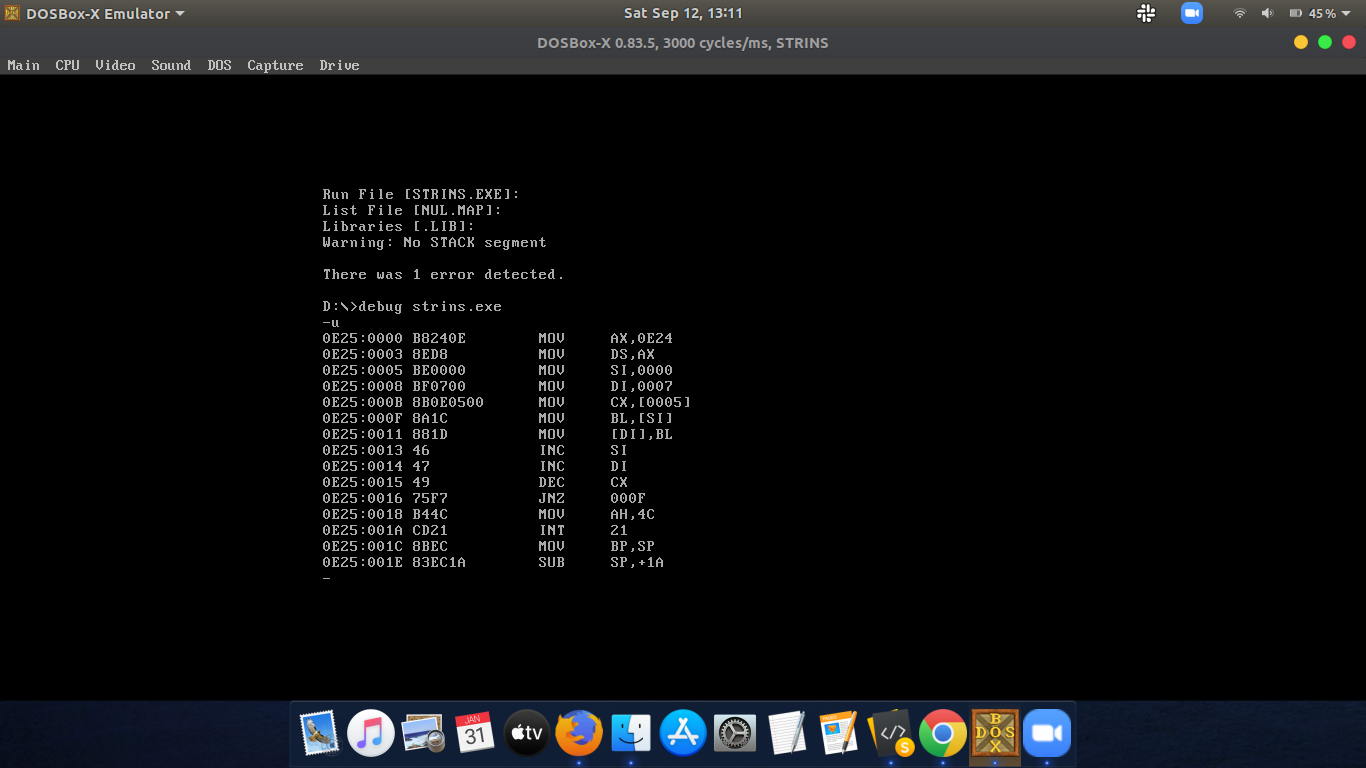
\includegraphics[trim = 100mm 60mm 200mm 120mm, clip, width = \textwidth]{Pics/StrinsUS.png}
\end{figure}
\subsubsection*{\textbf{Input and Output:}}
\begin{figure}[h]
    \centering
    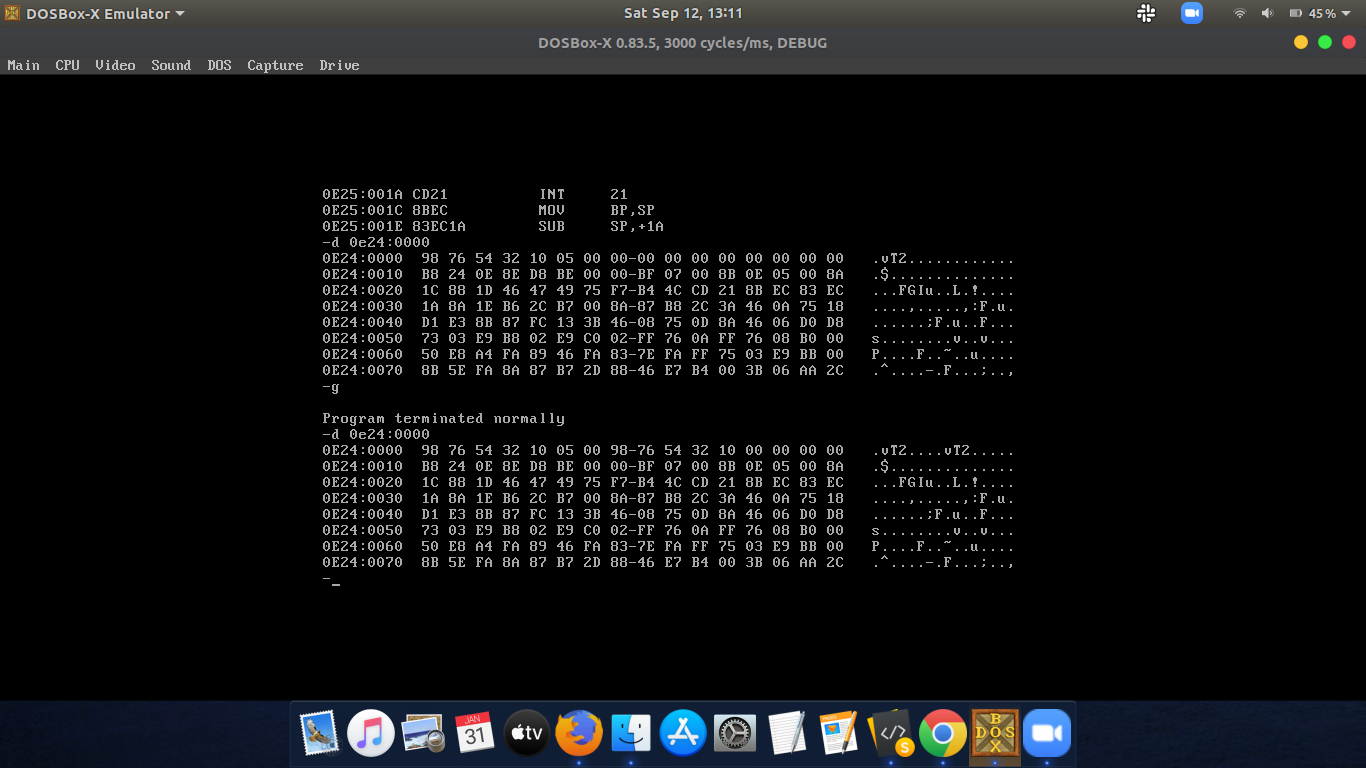
\includegraphics[trim = 100mm 60mm 100mm 80mm, clip, width = \textwidth]{Pics/StrinsIO.png}
    \caption{ \textbf{Input:} \emph{source:} 98 76 54 32 10H, \emph{dest:} 00 00 00 00 00H; \newline \hspace{1cm}
              \textbf{Output:} \emph{source:} 98 76 54 32 10H, \emph{dest:} 98 76 54 32 10H}
\end{figure}
\end{flushleft}
\end{document}